%! Author = charon
%! Date = 11/21/24
\section{Funktionsweise von Fuzzern}\label{sec:funktionsweise}
Die Funktionsweise eines Fuzzers kann im Wesentlichen fünf Komponenten~\ref{fig:struktur_fuzzing} zugeordnet werden:
\begin{itemize}
    \item \textbf{Initialisierung:} Der Fuzzer wird mit einer Menge von Testcases initialisiert, die an das SUT übergeben werden.
    \item \textbf{Dry Run:} Die Testcases werden an das SUT übergeben, um zu überprüfen, ob das SUT durch die Eingaben zum
        Absturz gebracht werden kann.
    \item \textbf{Mutator:} Der Mutator ist für die Generierung neuer Testcases verantwortlich.
    \item \textbf{Feedback:} Das Feedback des SUT wird verwendet, um die Testcases zu verfeinern.
    \item \textbf{System unter Test:} Stellt das zu testende Programm dar.
\end{itemize}
\begin{figure}
    \centering
    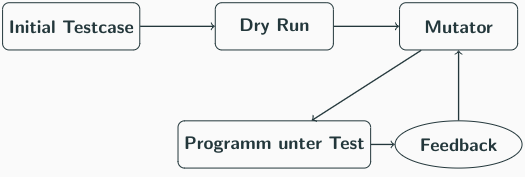
\includegraphics[width=\columnwidth]{res/Struktur_eines_fuzzing_prozesses}
    \caption[Struktur eines Fuzzing Prozesses]{
        Diese Abbildung zeigt den Ablauf eines Fuzzing Prozesses am Beispiel des Fuzzers AFL.
        Der Fuzzer verwendet die bereits gesammelten Testcases.
        Sie werden an das SUT in einer \enquote{Dry Run}-Phase übergeben, um zu überprüfen, ob es durch diese Eingaben
        bereits zum Absturz gebracht werden kann.
        Das Programm wird mit den Eingaben ausgeführt und die Ausgabe wird analysiert.
        Anhand der Analyseergebnisse wird ein Mutator verwendet, um neue Testcases zu generieren, die anhand der initial
        übergebenen Eingaben besonders tief in das Programm eingedrungen sind.
        Die vom Mutator generierten Eingaben werden an das SUT übergeben und das erlangte Feedback des SUT wird zur weiteren
        Verfeinerung der Eingaben verwendet.
        Somit bildet sich ein iterativer Prozess, der die Testcases immer weiter verfeinert.
    }\label{fig:struktur_fuzzing}
\end{figure}
